\chapter{Interferometric methods in tokamak plasmas}


\section{Gaussian beam diffraction}


\subsection{Definition of a Gaussian beam}
A Gaussian beam of angular frequency $\omega_0$
propagating along the $z$-axis
has an electric field
\begin{equation}
  E(\vect{r}, t)
  =
  E(\vect{r}) e^{-i \omega_0 t}
\end{equation}
with spatial dependence~\cite{siegman_lasers}
\begin{equation}
  E(\vect{r})
  =
  E_0
  \frac{w_0}{w(z)}
  \exp\left[ \frac{-\rho^2}{w(z)^2} \right]
  \exp\left\{ i \left[
    k_0 z
    +
    \frac{k_0 \rho^2}{2 R(z)}
    -
    \psi(z) \right] \right\}
  \label{eq:InterferometricMethods:Gaussian_beam}
\end{equation}
Here,
$\rho = (x^2 + y^2)^{1/2}$ is the transverse distance from the optical axis,
$w_0$ is the radius of the beam's waist, and
$k_0 = \omega_0 / c = 2 \pi / \lambda_0$ is the beam's wavenumber.
The beam's width $w(z)$, radius of curvature $R(z)$, and
Gouy phase $\psi(z)$ are defined as
\begin{align}
  w(z)
  &=
  w_0 \left[ 1 + \left( \frac{z}{z_R} \right)^2 \right]^{1/2}
  \label{eq:InterferometricMethods:Gaussian_beam_width}
  \\
  R(z)
  &=
  z \left[ 1 + \left( \frac{z_R}{z} \right)^2 \right]
  \label{eq:InterferometricMethods:Gaussian_beam_radius_of_curvature}
  \\
  \psi(z)
  &=
  \atan\left( \frac{z}{z_R} \right)
  \label{eq:InterferometricMethods:Gouy_phase}
\end{align}
where the Rayleigh range
\begin{equation}
  z_R \equiv \frac{\pi w_0^2}{\lambda_0}
  \label{eq:InterferometricMethods:Rayleigh_range}
\end{equation}
is the nominal division between the beam's
near-field ($|z| \ll z_R$) and far-field ($|z| \gg z_R$) behaviors.


\subsection{Kirchhoff diffraction theory}
A monochromatic scalar wave $U(\vect{r}) e^{-i \omega t}$ in vacuum
satisfies the Helmholtz equation
\begin{equation}
  (\nabla^2 + k^2) U = 0
\end{equation}
where $k = \omega / c$.
The Helmholtz-Kirchhoff integral theorem states
that the field at a point $P$ is
\begin{equation}
  U(P)
  =
  \frac{1}{4 \pi}
  \int_S \left[
    U \frac{\partial}{\partial n}\left(\frac{e^{i k s}}{s}\right)
    -
    \frac{e^{i k s}}{s} \frac{\partial U}{\partial n}
  \right] dS
  \label{eq:Helmholtz_Kirchhoff_integral_theorem}
\end{equation}
where $S$ is an arbitrary surface that encloses $P$,
$\vect{s}$ is the vector from point $P$ to differential area element $dS$,
$\vect{n}$ is the \emph{inward}-pointing normal of surface $S$, and
$U$ is assumed to be differentiable to second order within and on $S$
\cite{born_and_wolf}.
The relevant geometry is sketched
in Fig.~\ref{fig:InterferometricMethods:Kirchhoff_geometry}(a).

\begin{figure}
  \centering
  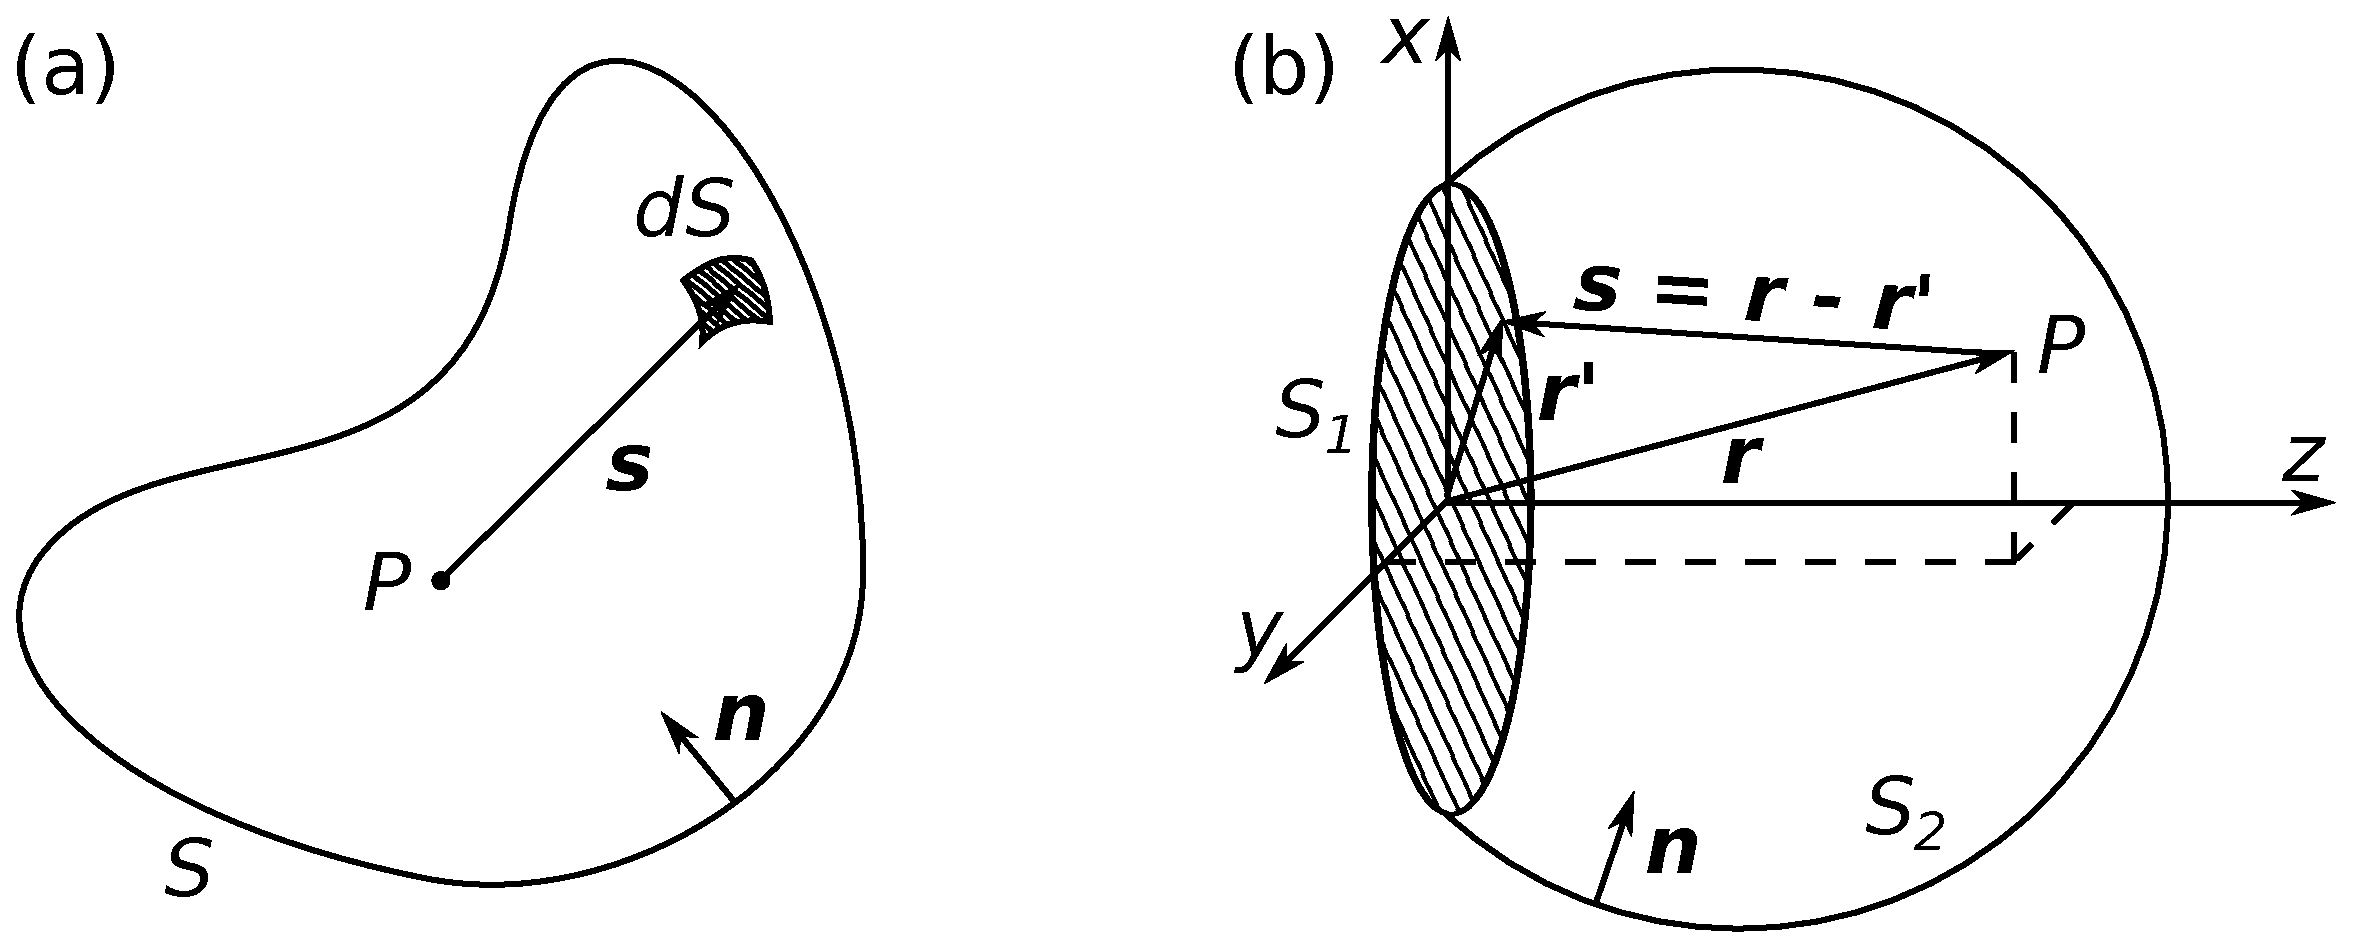
\includegraphics[width = \textwidth]{%
    Chapters/InterferometricMethods/figs/kirchhoff_geometry.eps}
  \caption{Geometry for Kirchhoff diffraction calculation.}
\label{fig:InterferometricMethods:Kirchhoff_geometry}
\end{figure}

To proceed with the diffraction calculation,
assume that the incident waves propagate in the $+z$-direction and
adopt the surface drawn
in Fig.~\ref{fig:InterferometricMethods:Kirchhoff_geometry}(b).
That is, $S = S_1 + S_2$,
where $S_1$ is a circle in the $(x, y)$-plane, and
$S_2$ is a spherical segment centered on the optical axis.
Now, assume that the incident waves were ``turned on''
at some finite time in the past, and
take the radius of $S_2$ to be large enough such that
none of the diffracted waves have had sufficient time to reach $S_2$,
i.e.\ $U \equiv 0$ on $S_2$.
(Of course, strictly speaking, the source's finite turn-on time
requires relaxation of the monochromatic assumption.
Finite turn-on time does not preclude a pseudo-monochromatic source, however,
and such a source is assumed hereafter).
Thus, the integral over $S_2$ vanishes, and
(\ref{eq:Helmholtz_Kirchhoff_integral_theorem})
reduces to an integral over $S_1$.


\subsection{Fraunhofer diffraction of a free-space Gaussian beam}
\subsection{Fraunhofer diffraction of a phase-modulated Gaussian beam}



\section{Laser-plasma interactions in a tokamak}
\begin{itemize}
  \item Cold-plasma dispersion relation and derivation of $N$
  \item Expected phase shifts in tokamak plasma
  \item Refraction
  \item Scattering/diffraction
\end{itemize}

\section{Interferometry}
\begin{itemize}
  \item Homodyne
  \item Heterodyne
  \item Vibrations
  \item $k$-response
\end{itemize}

\section{Phase contrast imaging}
\begin{itemize}
  \item Principle
  \item $k$-response
\end{itemize}


\bibliographystyle{plainurl}
\bibliography{references}
